% Generated by thesis/ch7/exp2/networks.py -- do not edit by hand.
\begin{sidewaysfigure}
  \centering
  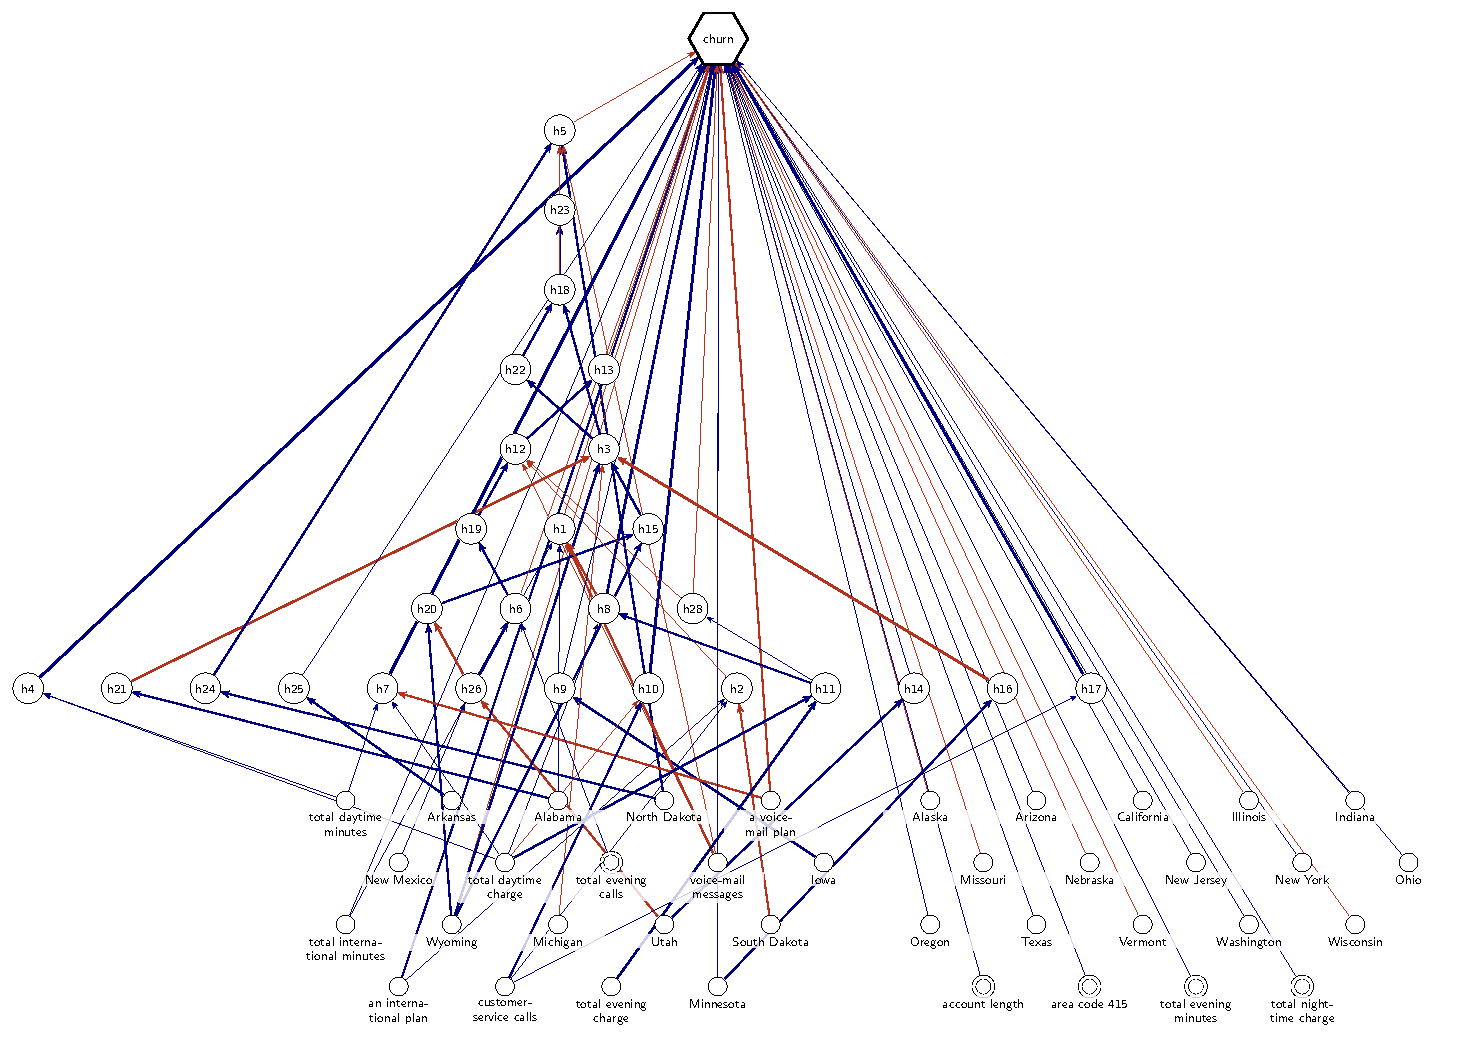
\includegraphics[width=\textheight,height=0.78\textwidth,keepaspectratio]{figures/exp2/networks/churn100-s1-raw}
  \caption{Churn, seed 1 (churn100-s1): the network as trained, before any explanation, in full. Inputs at the bottom (every input column its own node), hidden units by depth, the output at the top; 38 of 71 input columns are connected, with 27 hidden units and 92 enabled connections. Blue: positive weight (raises the score); red: negative weight (lowers it); thicker: larger weight. Orange outline and up arrow: raises the final prediction; teal and down arrow: lowers it; grey and double arrow: depends. Not used (no connection; 33 columns): Georgia, Hawaii, Idaho, Kansas, Kentucky, Louisiana, Massachusetts, Maryland, Maine, Mississippi, Montana, North Carolina, New Hampshire, Nevada, Oklahoma, Pennsylvania, Rhode Island, South Carolina, Tennessee, Virginia, West Virginia, Colorado, Connecticut, Washington DC, Delaware, Florida, area code 408, area code 510, total daytime calls, total night-time minutes, total night-time calls, total international calls and total international charge.}
  \label{fig:exp2-net-churn100-s1-raw}
\end{sidewaysfigure}
